\section{Analysis and Characterization of Memory Accesses in DNN}
\label{sec:char}
We analyze and characterize memory accesses in DNN and use the analysis results to drive our design.


\subsection{Profiling Framework}
\label{sec:profiling_framework}
%The major profiling challenge is to semantic difference between OS (page) and app (tensors)

%\textcolor{green}{paragraph: How OS level page access information are captured. TLB miss, PTE(page table entry) walk. }
We build a profiling framework for our study.
The profiling framework collects the following information: the number of main memory accesses per data object (tensor), data object size and lifetime. 


To collect the above information, the profiling framework includes the support at \textit{both} OS and TensorFlow runtime levels. At the OS level, \name collects the number of memory accesses at the page level. This is implemented by a software-only solution. In particular, when a page is tracked for access counting, \name sets a reserved bit (bit 51) in its PTE (i.e., poisoning PTE) and then flush the PTE from TLB. When the page is accessed, a TLB miss occurs and triggers a protection fault. \name uses a customized fault handler to count this page access, poison the PTE and flush it from TLB again to track next page access. Poisoning PET only happens during the profiling. After it, poisoning PTE and flushing TLB do not happen. 
%reserving the PTE bit and flushing PTE do not happen.


%\textcolor{red}{poisoning PTEs at the page table(i.e., setting PTE reserved bit) and then flushing the PTE from TLB. When the page be accessed again, a TLB miss occurs and triggers a protection fault. \name implement customized TLB miss handler to record page access information and poison this PTE again to keep recording the next of this page access. Note that \name profiling triggers a customized system call to start collect the number of memory access at page level. When the profiling finishes, another system call will be triggered and PTEs will no longer be poisoned. }

%To bridge the semantic gap between OS and application, each memory page has only one data object (but a data object can use more than one pages). 
To bridge the semantic gap between OS and application, each memory page has only one data object (but a data object can use more than one pages). \textcolor{dong}{This is implemented by making object allocation aligned with memory page.} Using this method, page-level profiling becomes data object-level profiling. Such memory allocation does not change memory access patterns captured by the hardware caching mechanism in the cache hierarchy, hence providing reliable estimation on memory accesses in main memory. Such memory allocation increases memory footprint. But it happens during the profiling phase of \name on slow memory. After the profiling phase, data objects are re-organized to reduce memory footprint and improve performance. Data reorganization happens \textit{during memory allocation}  (see Section~\ref{sec:dyn_profiling_data_org}), and hence does not stop the training process and does not impact performance. Also, the profiling method does not increase the consumption of fast memory. 


At the TensorFlow runtime level, \name leverages memory allocation and deallocation to get the size and lifetime of data objects. Furthermore, \name introduces an API that allows the user to annotate DNN to indicate the end of each layer in DNN.
%Furthermore, \name introduces two APIs that allow the user to annotate DNN to indicate the start and end of each layer in DNN. 
Based on the above infrastructure, \name is able to associate a data object with the DNN model topology of DNN (i.e., we can know which layer(s) a data object is alive). Setting up the association is helpful to direct data migration (Section~\ref{sec:adaptive_dm}). 

%%%%%%%%%%adding the reason for profiling at the OS level
\textcolor{dong}{The above profiling method is featured with a coordination between OS and TensorFlow runtime. Such a method provides accurate profiling, which is unachievable by TensorFlow runtime alone. In particular, OS allows us to track memory accesses filtered by processor caches; Working with the coordination between OS and TensorFlow runtime, we do not need to handle pointer aliasing commonly found in TensorFlow implementation. It is possible that we use \texttt{mprotect()} at the application level to track memory accesses to each data object without changing OS. However, given a large number of data objects, we have to extensively change TensorFlow implementation, which is not practical.}


%%%%\textcolor{jie}{
%%%The profiling framework involves OS level instead of only using application level data objects information because of following reason. 
%%%%Profiling at both OS level and application level is the optimal solution to get data object access information for DNN training workload because of following reasons. First, profiling at OS level can eliminates processor cache effect and obtain more accuracy result for page-based memory management. Second, profiling memory access in application level for DNN training workload is not trivial.  Frameworks(e.g., TensorFlow) and mathematical libraries(e.g., NumPy~\cite{oliphant2006guide}) for DNN training implemented with large amount of memory pointers and no runtime memory management(i.e., implemented by C/C++). Therefore, application level profiling needs large amount of pointer arithmetic to get the memory address where data objects access happens. Existing work~\cite{madt} explores profiling page access in user-space by using \textit{mprotect()} POSIX system call. However, DNN training workload involves large amount of data objects and each of them needs to make the system call to track page access, which is not practical.}

%%%%%%%%%%%%%%%%

Our profiling method uses only one %\textcolor{red}{one}
training step for profiling. During the profiling, \name captures each page read and write by repeatedly poisoning the page. This is expensive because of system calls and TLB misses. However, it does not lose profiling accuracy. Also, considering that a typical DNN training involves millions of training steps, the profiling overhead is easily amortized.  

The traditional profiling methods face a fundamental dilemma between profiling overhead and accuracy. In particular, frequently collecting memory access information brings high profiling accuracy at the cost of large runtime overhead, and vice versa~\cite{Thermostat:asplos17,RAMinate:socc16,heteros:isca17, sc18:wu, unimem:sc17}. Leveraging the repetitiveness of DNN training, \name breaks the dilemma, and enables both high profiling accuracy and low profiling overhead. 

%\textcolor{green}{paragraph: Existing work use OS level profile use sampling based approach intercept TLB miss to capture hot and code pages.}

%\textcolor{green}{paragraph: TensorFlow provides profiling API to profile the input and output tensor for operations. The information is course-gained and not suitable for migration: (1) lack of tensor access info which has been used instead of operations. (not work for short-lived tensor). (2) lack of tensor location information. tensorflow profiling API only provide the information of the pointer points to tensor instead of the real address of tensors. The pointer information is not suitable for page migration. }

%\textcolor{green}{paragraph: app level profiling: profiling tensor access in app runtime ask for a lot of engineering efforts. need to intercept every tensor access in every operation. Not practical, not general.}

%\textcolor{green}{paragraph: Our profiling method. We adopt the combination of profiling in both OS level and app level. In app level we intercept tensor allocator/deallocator to get tensor size and lifetime information; In OS level we poison PTE to trigger protection fault and record every page access.}

%\textcolor{green}{paragraph: Due to the predicative of ML model, profiling one training step without sampling can have more accurate result. Profiling happens on slow memory.

\subsection{Profiling Results and Analysis}
\label{sec:profiling_results}


\begin{figure}[!t]
\centering
%\vspace{-10pt}
%\includegraphics[width=0.48\textwidth]{ASPLOS2020_Jie/figures/f1_3edit.pdf}
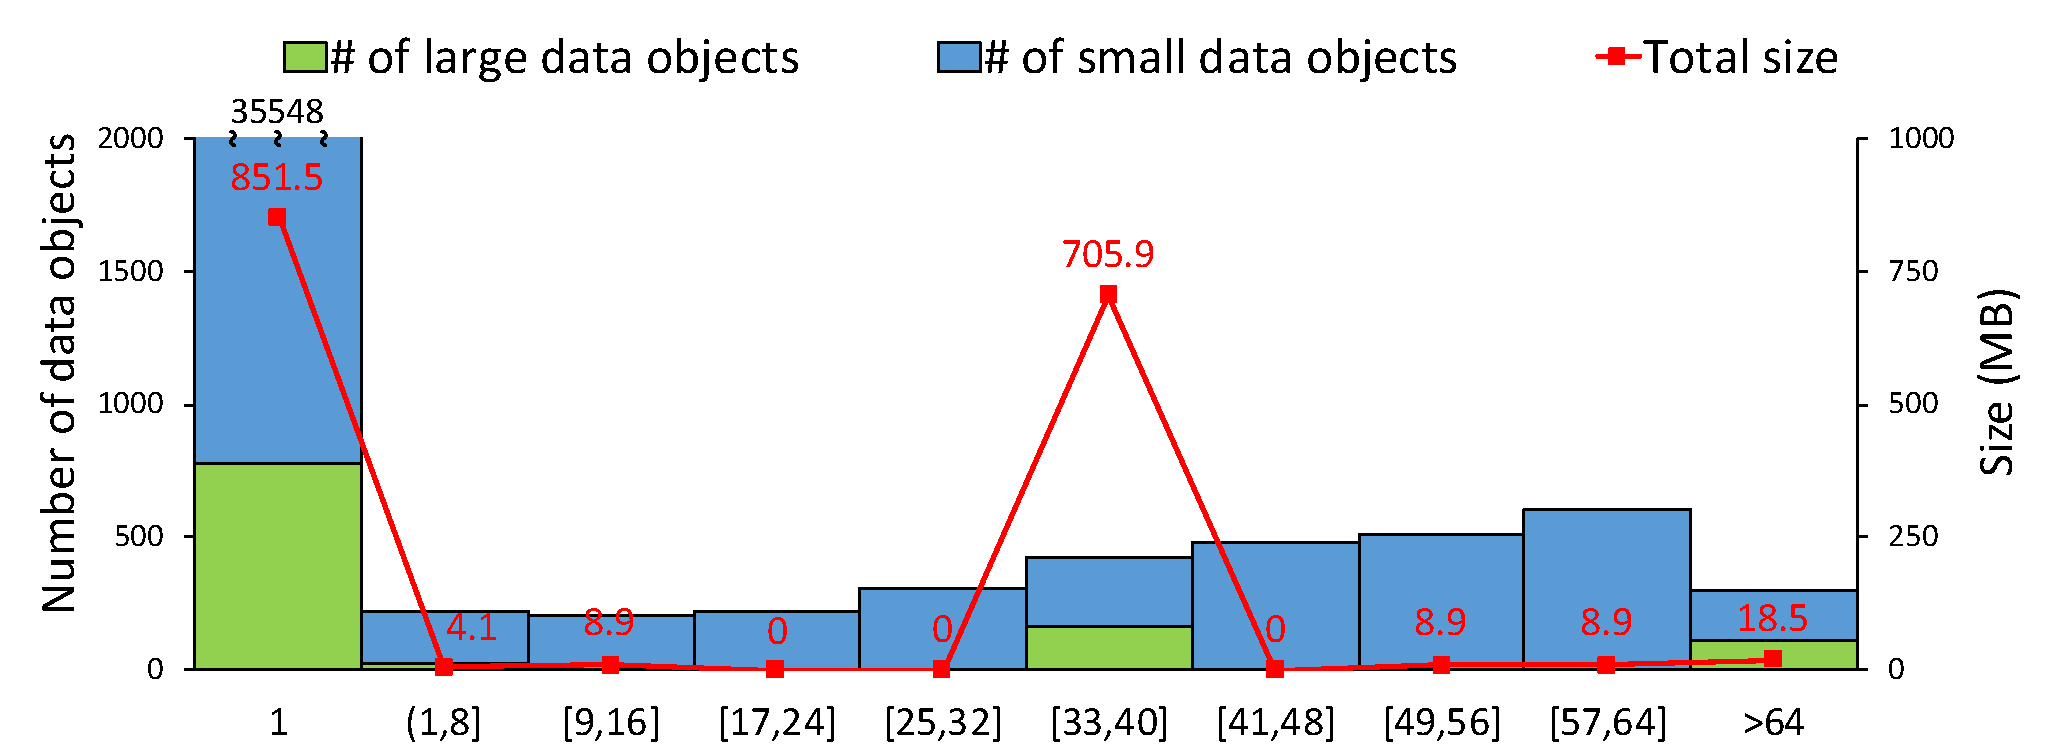
\includegraphics[width=0.48\textwidth]{figures/figure1.pdf}
%\vspace{-10pt}
%\caption{\name tensor access histogram.  x-axis shows tensor access frequency and y-axis shows the number of tensors.}
\caption{Distribution of lifetime of data objects and their sizes for ResNet\_v1-32. Each small data object is smaller than 4KB; Each large data object is no smaller than 4KB. ``>64'' means that the data object survives more than one forward and backward pass (one training step).}
%\textcolor{red}{need to conform}}
%\vspace{-10pt}
\label{fig:fig_lifetime}
\end{figure}


\textcolor{dong}{We profile DNN models listed in Table~\ref{tab:models} and have the following observations.}


We use the profiling framework to study data objects and their access patterns in DNN. We report profiling results for one training step in this section.

Figure~\ref{fig:fig_lifetime} shows the distribution of lifetime of data objects and their accumulated sizes for ResNet\_v1-32 (the configuration of training is in Table~\ref{tab:models}). ResNet\_v1-32 has 64 layers (in a forward and backward pass).  %(\textcolor{dong}{each residual block has two layers})}.  
%and \textcolor{orange}{consumes 6GB memory. 
A data object is alive after it is allocated and before it is freed. The lifetime of a data object is defined in terms of number of layers where the data object is alive.
%The lifetime of a data object is defined from memory allocation to memory free. The lifetime is shown in terms of layers in Figure~\ref{fig:fig_lifetime}. 
Figure~\ref{fig:fig_lifetime} shows that 92\% of data objects have lifetime no longer than one layer. Among those short-lived data objects, 98\% of them is small data objects (smaller than 4KB). 
%but their total size is not big (\textcolor{red}{xxx} MB).  

%\textcolor{red}{Figure: distribution of lifelime and size. Purpose of this figure: most tensors have short live.}
\begin{comment}
\pgfplotsset{width=8cm,compat=1.8, 
     legend style={
      fill,
      at={(0.50,-0.1)},
      legend columns=1,
      legend cell align=left,
      anchor=north
      },}
    %  ylabel shift = -8 pt,
\begin{figure}
\resizebox{0.5\textwidth}{0.3\textwidth}{
\begin{tikzpicture}
\begin{axis}[axis y line*=left,ylabel={Number of tensors},ybar stacked, ylabel style={font=\large},bar shift=0pt,bar width=1,ymin=0,ymax=2000, xmin=0,xmax=10,
xtick={1,2,3,4,5,6,7,8,9, 10},
xticklabels={1,8,16,24,32,40,48,56,64},xtick style={draw=none},ytick style={draw=none},]
%scaled y ticks=base 10:-2]
\addplot [fill=RYB2] coordinates
{(0.5,780) (1.5,24) (2.5,4) (3.5,0) (4.5,0) (5.5,168) (6.5,0) (7.5,4) (8.5,4) (9.5, 110)};\label{lb} 
\addplot [fill=RYB1]coordinates
{(0.5,34768) (1.5,195) (2.5,202) (3.5,221) (4.5,305) (5.5,259) (6.5,476) (7.5,507) (8.5,604) (9.5, 192)};\label{sb}
\end{axis}
\begin{axis}[axis y line*=right,
%scaled y ticks=base 10:-2,
   xticklabels={},xtick style={draw=none},
  ymin=0, ymax=1000,
   %ytick={0, 0.25, 0.5, 0.75, 1.0},
   ylabel={Mem size (MB)},ylabel style={font=\large},
   nodes near coords,
        every node near coord/.append style={font=\normalsize,text=black},
   ytick style={draw=none}]
\addlegendimage{/pgfplots/refstyle=lb}
\addlegendentry{Number of large data objects}
\addlegendimage{/pgfplots/refstyle=sb}
 \addlegendentry{Number of small data objects}
   \addplot[draw=red,mark=square] plot coordinates{
      (0.5,851.5)(1.5,4.1)
      (2.5,8.9) (3.5,0.1) (4.5,0.1)
      (5.5,705.9) (6.5,0.1) (7.5,8.9) (8.5,8.9)
      (9.5,18.5)
      };
    \addlegendentry{Total mem size}
   \end{axis}
 \node [red] at (0.4,5.5) {35548};
\end{tikzpicture}
}
\caption{Distribution of lifetime of data objects and their sizes for ResNet-32.}
\label{fig:fig_lifetime}
\end{figure}
\end{comment}



\textbf{Observation 1}: There are a large number of small data objects with short lifetime in DNN workloads.

In the rest of the paper, we define short-lived data objects as those with lifetime no longer than one layer.

%\textcolor{dong2}{The size of memory space for short-lived data objects is small, and typically bounded by a few GB.} 

\begin{figure}[!t]
\centering
%\vspace{-5pt}
%\includegraphics[width=0.48\textwidth]{figures/tensor_access.pdf}
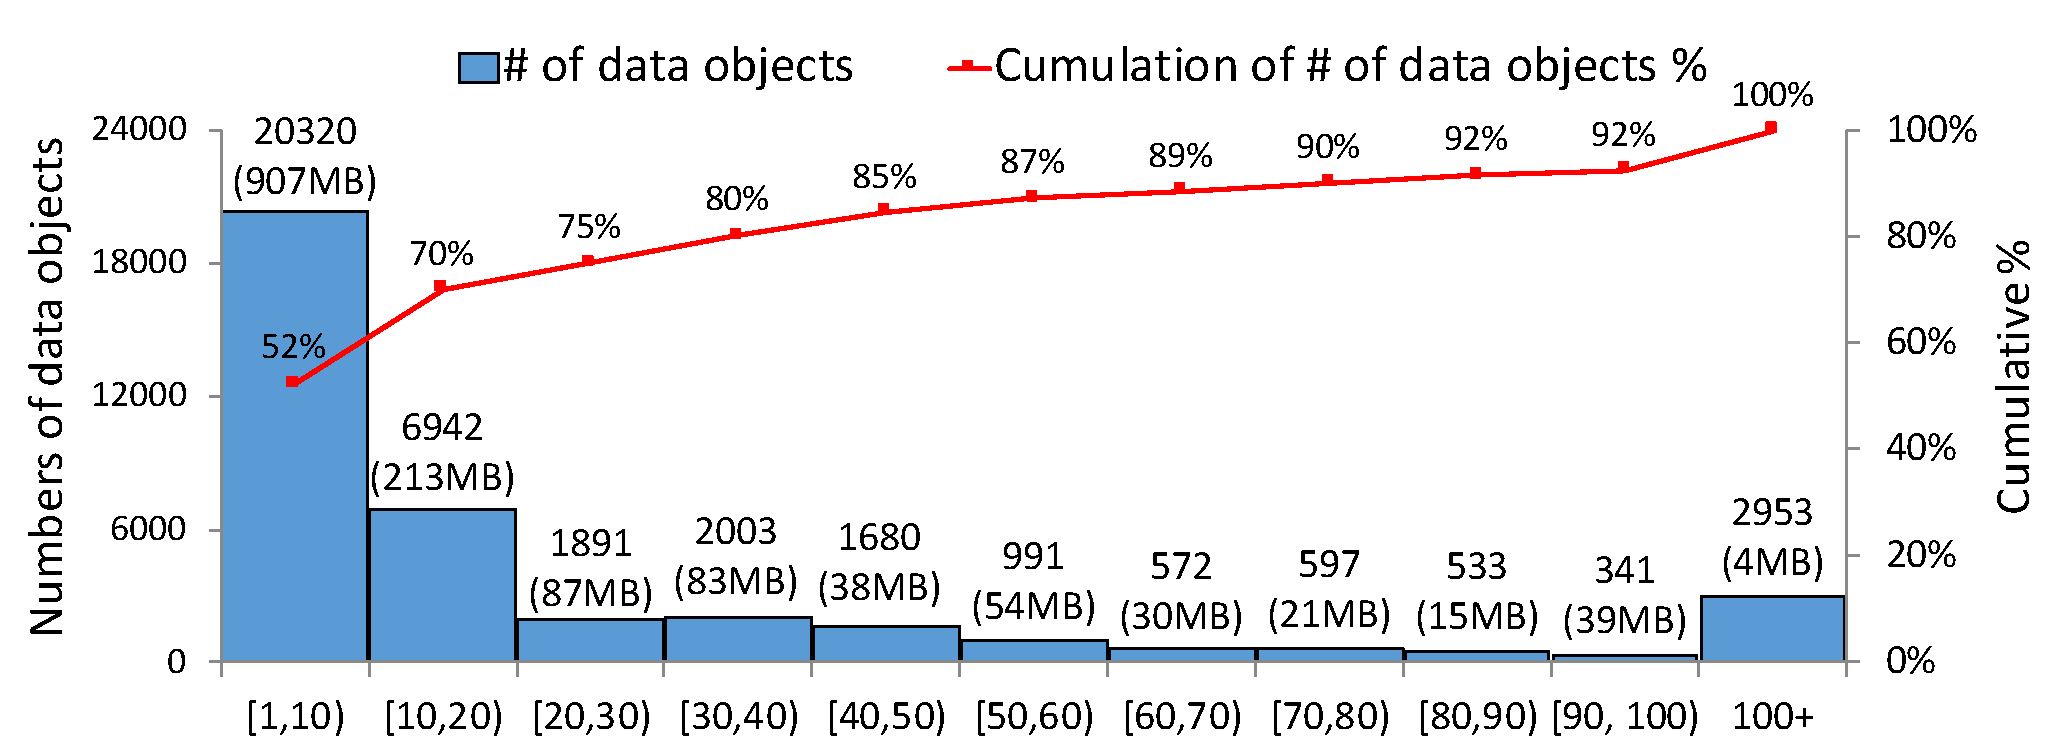
\includegraphics[width=0.48\textwidth]{figures/figure2.pdf}
%\vspace{-20pt}
%\caption{\name tensor access histogram.  x-axis shows tensor access frequency and y-axis shows the number of tensors.}
\caption{Distribution of the number of main memory accesses at the data object level.}
%\vspace{-5pt}
\label{fig:tensor_access}
\end{figure}

\begin{figure}[!t]
\centering
%\vspace{-20pt}
%\includegraphics[width=0.48\textwidth]{figures/small_tensor_access.pdf}
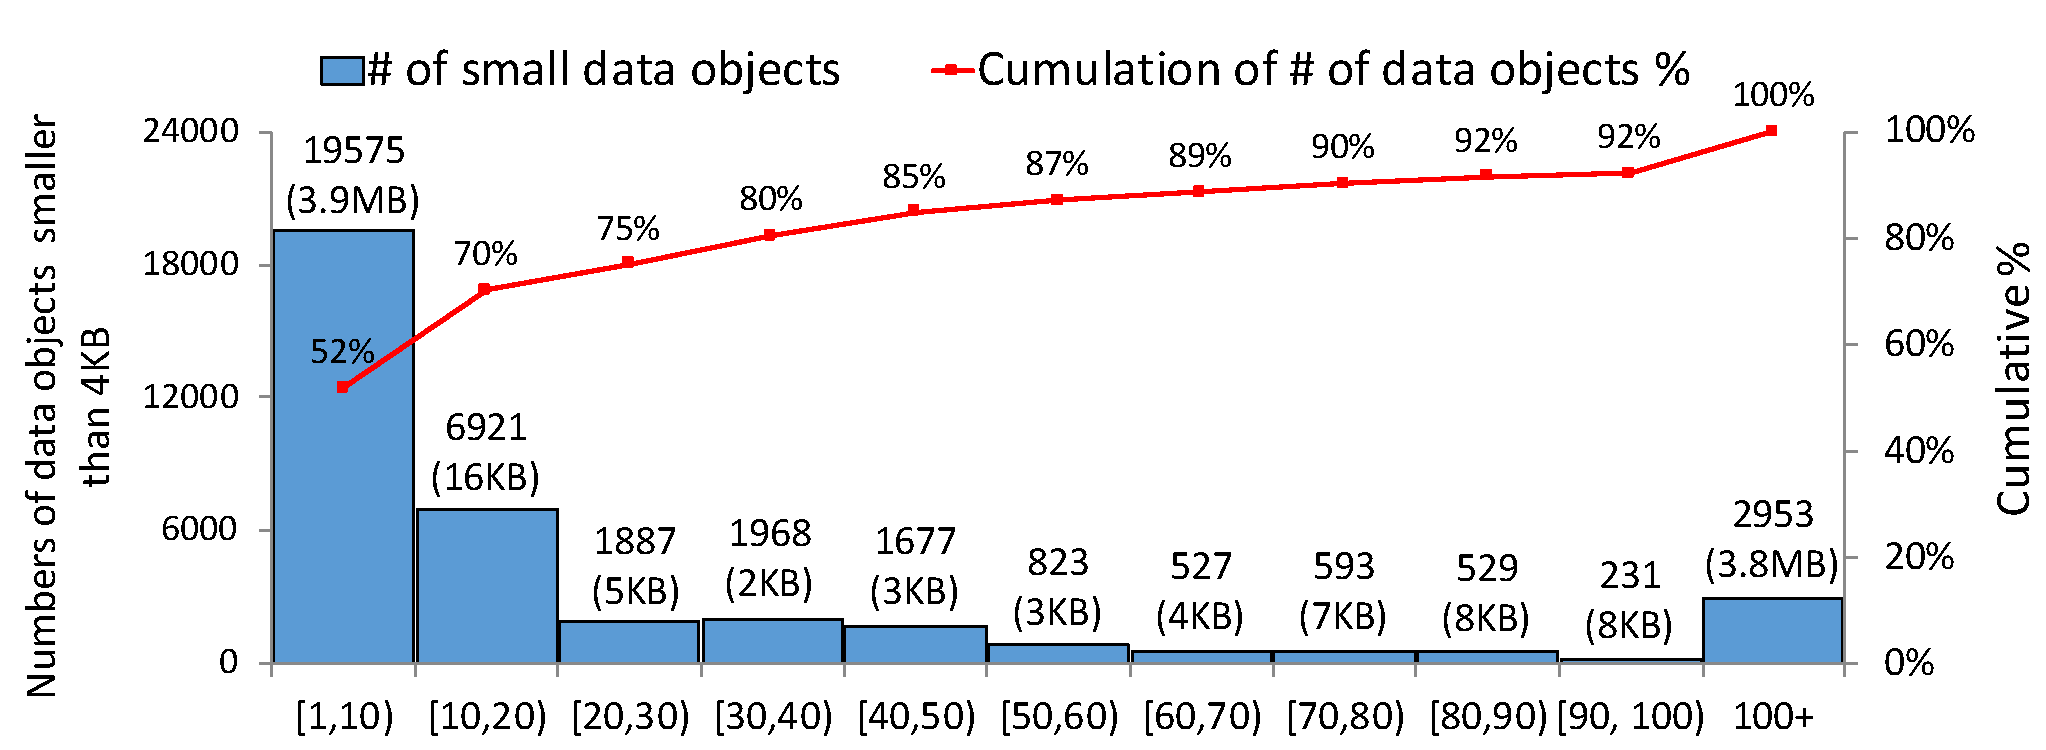
\includegraphics[width=0.48\textwidth]{figures/figure3.pdf}
%\vspace{-25pt}
%\caption{\name tensor access histogram.  x-axis shows tensor access frequency and y-axis shows the number of tensors.}
\caption{Distribution of the number of main memory accesses at the data object level for small data objects (each is smaller than 4KB).}
%\vspace{-10pt}
\label{fig:small_tensor_access}
\end{figure}

%\textcolor{red}{Figure: show the distribution of number of memory accesses to smaller tensors (less than one mem page). Show how many pages those tensors use. Purpose of this figure: (1) page-level false sharing exists (define false-sharing); (2) there is opp to reduce the fast mem size}

Figure~\ref{fig:tensor_access} shows the distribution of the number of main memory accesses at the data object level. 
%We collect the data in the figure after data re-organization. 
%%%\textcolor{green}{We collect the data in figure by allocating each memory page has only one data object.}
The figure shows that a large number of data objects (52.3\% of data objects, using 907 MB, which is 54\% of total memory pages) are accessed less than 10 times. Among them, 98\% of them are small (\textcolor{dong2}{less than 4KB}) and use only 3.9 MB in total, shown in Figure~\ref{fig:small_tensor_access}. On the other hand, some data objects are frequently accessed (having >100 accesses), taking only 4 MB (0.2\% of total memory pages). They are the candidates to be placed into fast memory, and their size is a small portion of total memory pages. 


\begin{comment}
\begin{figure}[!t]
\centering
%\vspace{-20pt}
\includegraphics[width=0.48\textwidth]{figures/tensor_access.pdf}
%\vspace{-20pt}
%\caption{\name tensor access histogram.  x-axis shows tensor access frequency and y-axis shows the number of tensors.}
\caption{Distribution of the number of main memory accesses at the data object level.}
%\vspace{-5pt}
\label{fig:tensor_access}
\end{figure}

\begin{figure}[!t]
\centering
%\vspace{-20pt}
\includegraphics[width=0.48\textwidth]{figures/small_tensor_access.pdf}
%\vspace{-25pt}
%\caption{\name tensor access histogram.  x-axis shows tensor access frequency and y-axis shows the number of tensors.}
\caption{Distribution of the number of main memory accesses at the data object level for small data objects (each is smaller than 4KB).}
%\vspace{-10pt}
\label{fig:small_tensor_access}
\end{figure}
\end{comment}
\textbf{Observation 2}: The uneven distribution of hot and cold data objects in DNN provides opportunities for data management. 

\begin{table}[!tbh]
%\vspace{-10pt}
%\small
\centering
\caption{Memory consumption (in one training step) in the original execution and using ``one data object per page'' in the profiling step. ``prof.'' stands for ``profiling''.} 
\label{tab:mem_consume}
\begin{tabular}{|c|c|c|}
\hline
memory consumption                                                       & in prof. & Orig. exe.  \\ \hline
all data objects                                                         & 1.97 GB   & 1.57 GB    \\ \hline
\begin{tabular}[c]{@{}c@{}}data objects \\ smaller than 4KB\end{tabular} & 152 MB    & 0.45 MB    \\ \hline
\end{tabular}
\end{table}

%\textcolor{red}{Figure: show the distribution of number of memory accesses at page level. Purpose of this figure: show the difference between page-level and tensor-level profiling.}

\textcolor{dong2}{Table~\ref{tab:mem_consume} shows memory consumption for two cases: (1) the original execution and (2) using ``one data object per page'' in the profiling step. In the original execution, small data objects takes only 0.45MB, but using one data object per page, they take 152 MB.} This indicates that small data objects commonly share pages with other data objects. 

Figure~\ref{fig:size_diff} shows the distribution of the number of main memory accesses at different levels, including at the data object level already shown in Figures~\ref{fig:tensor_access} and~\ref{fig:small_tensor_access}, and page level in the original execution. The figure shows that for less frequently accessed data objects (having 1-10 accesses), the total size of data objects (907 MB) is larger than the total page size (763 MB) in \textcolor{dong2}{the original execution}. 

This result is interesting, because if alive data objects fall into the same pages, the size of the data objects should be smaller than or equal to the size of pages.  
%\textcolor{green}{if data objects with similar access time falling into the same pages, the size of the data objects should be smaller than or equal to the size of pages. }
Our result is against the above rationale, which suggests that some data objects actually do not fall into those 763MB-pages \textcolor{dong2}{in the original execution}. This means \textcolor{dong2}{in the original execution}, those data objects fall into other pages that are counted as more frequently accessed. In other words, those data objects share the pages with other data objects that may have different preference for data placement. We refer to the above result as \textit{page-level false sharing} in the rest of the paper. 




%This indicates that some of these data objects are placed into the same page. Since the data objects in the same page can be accessed at different execution time, such a memory page can be . An example of this case is xxxx. We call this case page-level false sharing in the rest of the paper.




%%We notice that 48\% of pages is not frequently accessed (less than ten times). %Those pages have great potential to be placed in slow memory in most of the training time. Those frequently accessed pages (having >500 accesses) only take about \textcolor{red}{xxx} MB (3.3\% of total memory pages). This result is different from Figure~\ref{fig:tensor_access} at the tensor level. page-level false sharing.
%Those hot pages are candidates to be placed into fast memory. The small size of those hot pages shows great potential to use a small fast memory.

\begin{comment}
\begin{figure}
\centering
%\vspace{-20pt}
\includegraphics[width=0.48\textwidth]{figures/page_access.pdf}
%\vspace{-25pt}
\caption{Distribution of the number of main memory accesses at the page level without data re-organization.}
%\caption{x-axis shows the page access frequency and the y-axis shows the number of pages.}
%\vspace{-10pt}
\label{fig:page_access}
\end{figure}
\end{comment}

\textbf{Observation 3}: Page-level false sharing exists in DNN. The page-level profiling (not data object-level) for data management can be misleading because of page-level false sharing. 

%\textcolor{red}{Figure: show the number of tensors and their sizes per layer. Purpose of this figure: to show the variance of tensor usages across layers.}

\begin{figure}[!th]
\centering
%\vspace{-20pt}
%\includegraphics[width=0.48\textwidth]{figures/mem_size.pdf}
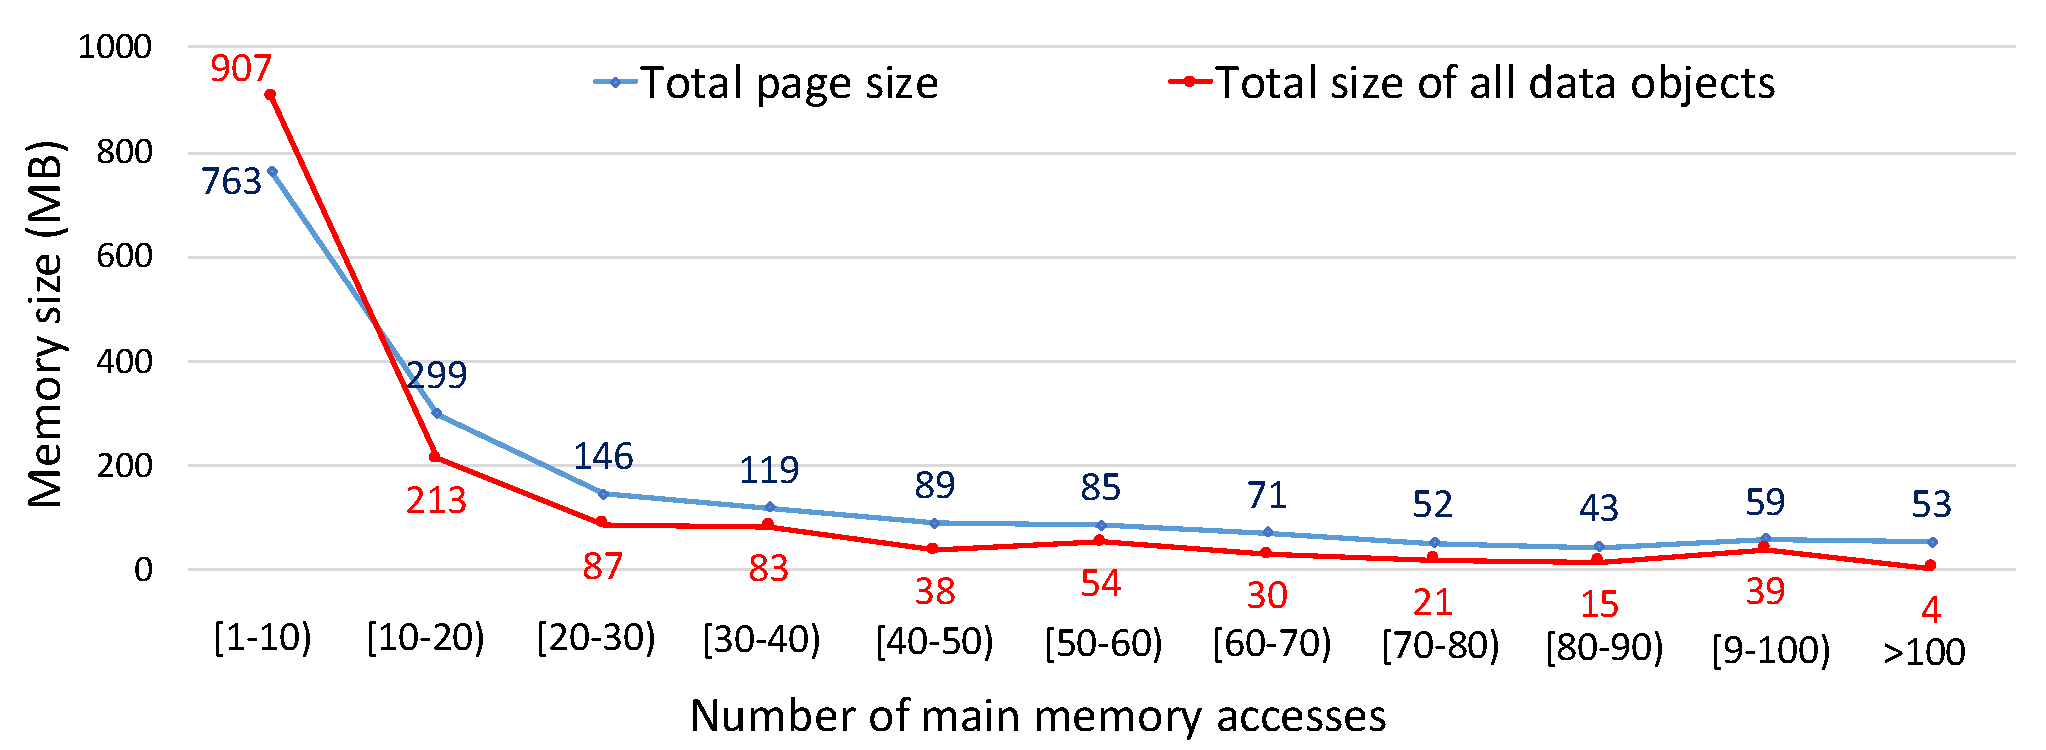
\includegraphics[width=0.48\textwidth]{figures/figure4.pdf}
%\vspace{-25pt}
%\caption{\name tensor access histogram.  x-axis shows tensor access frequency and y-axis shows the number of tensors.}
\caption{Distribution of the number of main memory accesses at the levels of pages (in the original execution), data objects, and small data objects.}
%\vspace{-10pt}
\label{fig:size_diff}
\end{figure}



%\textcolor{green}{Figure~\ref{fig:page_access} shows main memory page access distribution in page level. More than 50\% of pages access time is less 10 times. Figure~\ref{fig:size_diff} shows the accumulated size with different profiling method. Page-level profiling can over-estimate data object access because of false-sharing.}



%%%%%%%%%%%%%%%%%%%%%new example
\begin{figure}
\centering
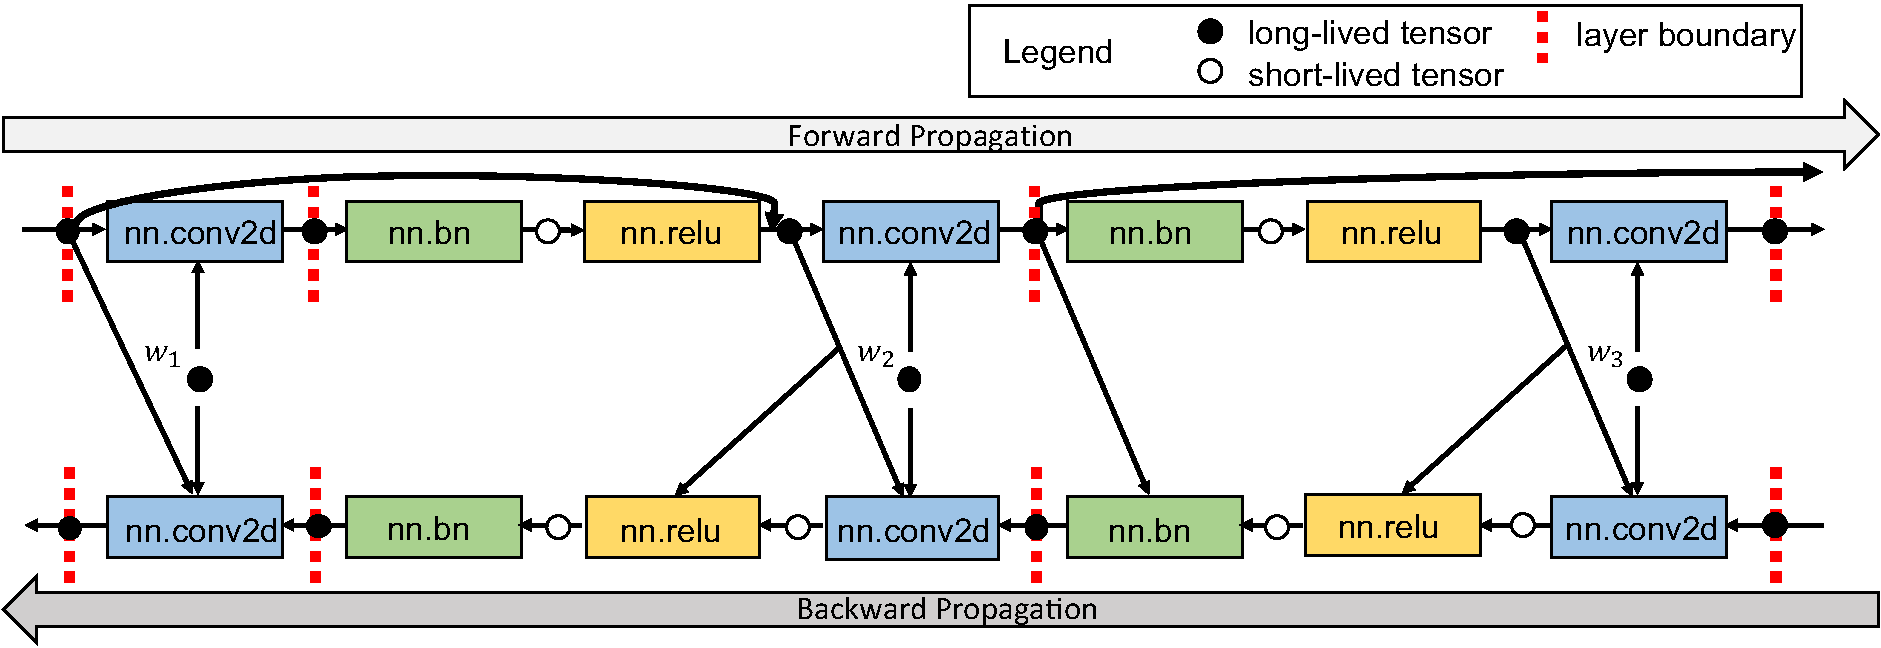
\includegraphics[width=0.48\textwidth]{figures/tensor_usage.pdf}
\caption{\textcolor{jie}{Data object access example in ResNet}.}
\label{fig:tensor_usage}
\end{figure}
\begin{figure}
\centering
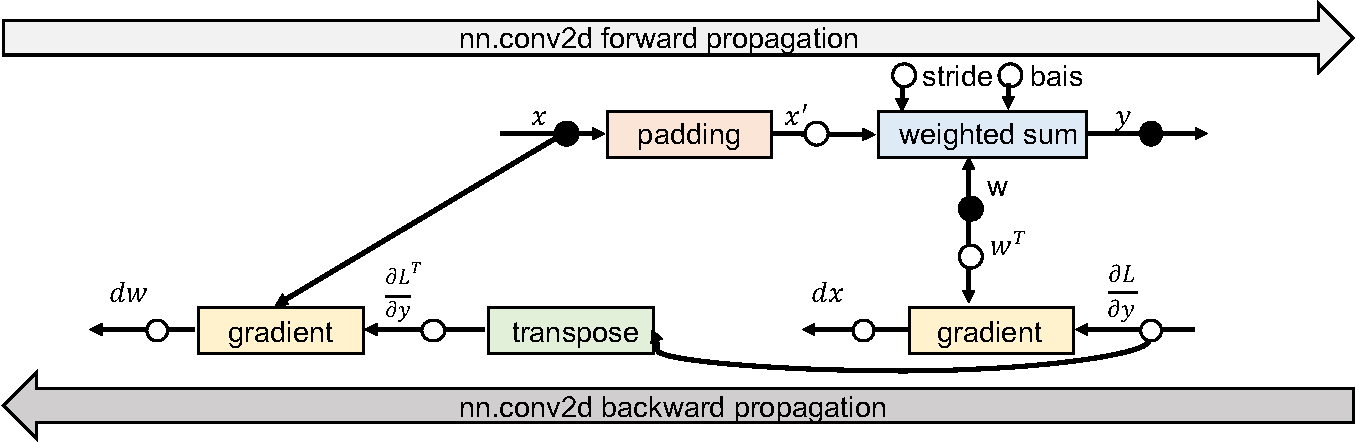
\includegraphics[width=0.48\textwidth]{figures/conv_tensor_usage.pdf}
\caption{\textcolor{jie}{Data object access example in tensorflow Conv2d operation }.}
\label{fig:conv_tensor_usage}
\end{figure}
\textcolor{jie}{
\textbf{Example. }
%%%%\name treats forward and backward pass into different layers. Data object in different layer has different reuse. 
Computation graph declaration and execution are separated in DNN training framework. 
For example, TensorFlow codes contains two parts, graph building and session running. 
Data objects keep allocating and deallocating during computation graph execution. Current execution operations consumes  
Figure~\ref{fig:tensor_usage} illustrates data objects(i.e., tensors) access details in ResNet~\cite{resnet_32} training.
%%%Each layer direct consumes data objects produced by previous layer. If the data object does not be access again, the data object will be deallocated to save memory space.
Data objects severs for different proposes
Long-lived data objects access multiple times during the training process, but the reuse of the long-lived data objects are various. 
}

\textcolor{jie}{Further, we analysis data object usage inside of an operation. 
Figure~\ref{fig:conv_tensor_usage} shows the data object access for Conv2D operation in TensorFlow. Instead of each operation, there are large amount of data objects for intermediate results. In figure~\ref{fig:conv_tensor_usage}, the memory for output of padding and transpose are allocated before the convolution operation begins and deallocated after this operation finished. }